\usetikzlibrary{arrows.meta, decorations.markings, patterns, calc, decorations.pathmorphing}

\newcommand{\nib}[3]{% #1 = anchor point, #2 = fill color
  \draw[fill=#2, rotate=#3] (#1) ++(0,0.15) arc (90:-90:0.15);
}

\begin{figure}
    \centering
    \begin{adjustbox}{width=\linewidth}
    \tikzset{
    polarizer/.style={draw, fill=orange!10, minimum width=1.5cm, minimum height=0.3cm},
    crystal/.style={draw, fill=teal!20, minimum width=0.4cm, minimum height=1.5cm},
    mirror/.style={draw, fill=black!60, minimum width=0.1cm, minimum height=1.5cm, inner sep=0},
    beam/.style={red, thick, decoration={markings, mark=at position 0.5 with {\arrow{Stealth}}}, postaction={decorate}},
    laser/.style={draw, fill=blue!20, minimum width=2cm, minimum height=1cm},
    coupler/.style={draw, fill=violet!30, minimum width=0.5cm, minimum height=0.8cm},
    fiber/.style={thick, violet},
    }

    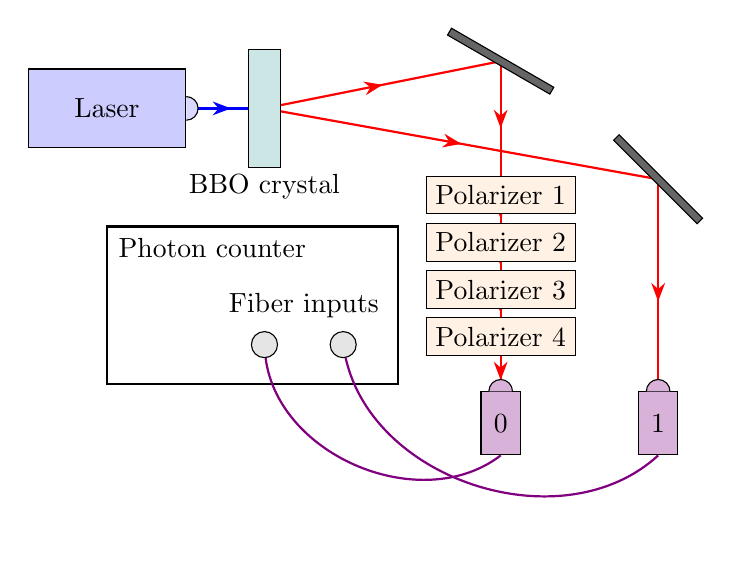
\begin{tikzpicture} 
    % beam path
    
    \draw[beam, blue] (4.15,0) -- (5,0);

    \draw[beam] (5,0) -- (8,0.6);
    \draw[beam] (8,0.6) -- (8, -1.1);
    \draw[beam] (8,-1.1) -- (8, -1.7);
    \draw[beam] (8,-1.7) -- (8, -2.3);
    \draw[beam] (8,-2.3) -- (8, -2.9);
    \draw[beam] (8,-2.9) -- (8, -4);

    \draw[beam] (5,0) -- (10,-0.9);
    \draw[beam] (10,-0.9) -- (10,-4);

    % optical elements
    \node[laser] (src)  at (3,0) {Laser};
    \nib{src.east}{blue!15}{0}

    \node[crystal] (crys2) at (5, 0) {};
    \node[anchor=north, inner sep=2pt] at (crys2.south) {BBO crystal};

    \node[mirror, rotate = 60] at (8,0.6) {};
    \node[polarizer, rotate = 0] at (8, -1.1) {Polarizer 1};
    \node[polarizer, rotate = 0] at (8, -1.7) {Polarizer 2};
    \node[polarizer, rotate = 0] at (8, -2.3) {Polarizer 3};
    \node[polarizer, rotate = 0] at (8, -2.9) {Polarizer 4};
    \node[coupler] (coupler0) at (8, -4) {0};
    \nib{coupler0.north}{violet!30}{90}

    \node[mirror, rotate = 45] at (10,-0.9) {};
    \node[coupler] (coupler1) at (10, -4) {1};
    \nib{coupler1.north}{violet!30}{90}

    \draw[thick, black] (3,-1.5) rectangle (6.7,-3.5);
    \node[anchor=north west, inner sep=4pt] at (3,-1.5) {Photon counter};

    \node[draw, fill=gray!20, circle, minimum size=0.2cm] (c0) at (5,-3) {};
    \node[draw, fill=gray!20, circle, minimum size=0.2cm] (c1) at (6,-3) {};
    \node at (5.5,-2.5) {Fiber inputs};

    \draw[fiber] (coupler0.south) to[bend left=60] (c0);
    \draw[fiber] (coupler1.south) to[bend left=60] (c1);

    \end{tikzpicture}
    \end{adjustbox}

    \caption{Experimental setup. The laser diode outputs \qty{405}{\nano\meter} horizontally-polarized light, which passes through a nonlinear down-conversion crystal (beta-barium borate, or BBO), which causes the incident photons to undergo spontaneous parametric down-conversion \cite{qutoolsgmbhQuEDManual2021}. This then generates pairs of horizontally-polarized \qty{810}{\nano\meter} photons, which then are separated into two arms. The photon in arm 0 passes through 4 successive polarizers, whereas the photon in arm 1 passes through free space. At the end of each arm, the photons are coupled into optical fibers and led into the input of a photon counter that detects coincident photons.}\label{fig:expsetup}
\end{figure}